\section{Discussion}

When looking at Figure \ref{fig:noNS_perf} we observe that all portfolio considered perform better than the inverse volatility benchmark as well as the equally weighted benchmark. Specifically, the portfolios return monthly geometric average total return between 0.43\% and 0.54\% while the the benchmarks achieve 0.3\% in the case of the inverse volatility benchmark and 0.45\% in the case of the equally weighted benchmark. In terms of Geometric Sharpe Ratio the portfolio using the "ward" method is by far the most appealing one, with 0.86, although it falls short of the inverse volatility benchmark which achieves a Geometric Sharpe Ratio of 1.02 due to its far lower standard deviation. It is of particular interest to notice that all four portfolios exhibit negative skewness and kurtosis below 3. Furthermore, we observe the same pattern when we consider the News Sentiment enhanced portfolios.

As the portfolio based on the "ward" method is the clear winner between the four portfolios consider, we focus our attention now to the comparison of the portfolio with and without News Sentiment. Following the approach of \citet{enhPortOpti} we run our benchmark for different starting month in order to check for robustness. The result is displayed in Figure \ref{fig:noNS_perf}. Unfortunately we cannot draw a conclusion on the effectiveness of the News Sentiment enhancement as there is no clear winner between the two approaches. 

Motivated by the fact that even the magnitude of the performance of the two portfolios varies across the chosen starting month of the portfolio we run 12 backtest, one for each month of the year. This robustness check is done for both with or without News Sentiment enhancement. Results are displayed in Appendix 1. It can be observed that the portfolios are not robust and that their performance varies with the month selected. However, it can be seen that overall "ward" performs the best when there is no News Sentiment enhancement while "single" performs the best among the News Sentiment enhanced portfolios.


\newpage
\begin{figure}[H] % "[t!]" placement specifier just for this example
\centering

\begin{subfigure}{0.8\textwidth}%{0.48\textwidth}
\centering
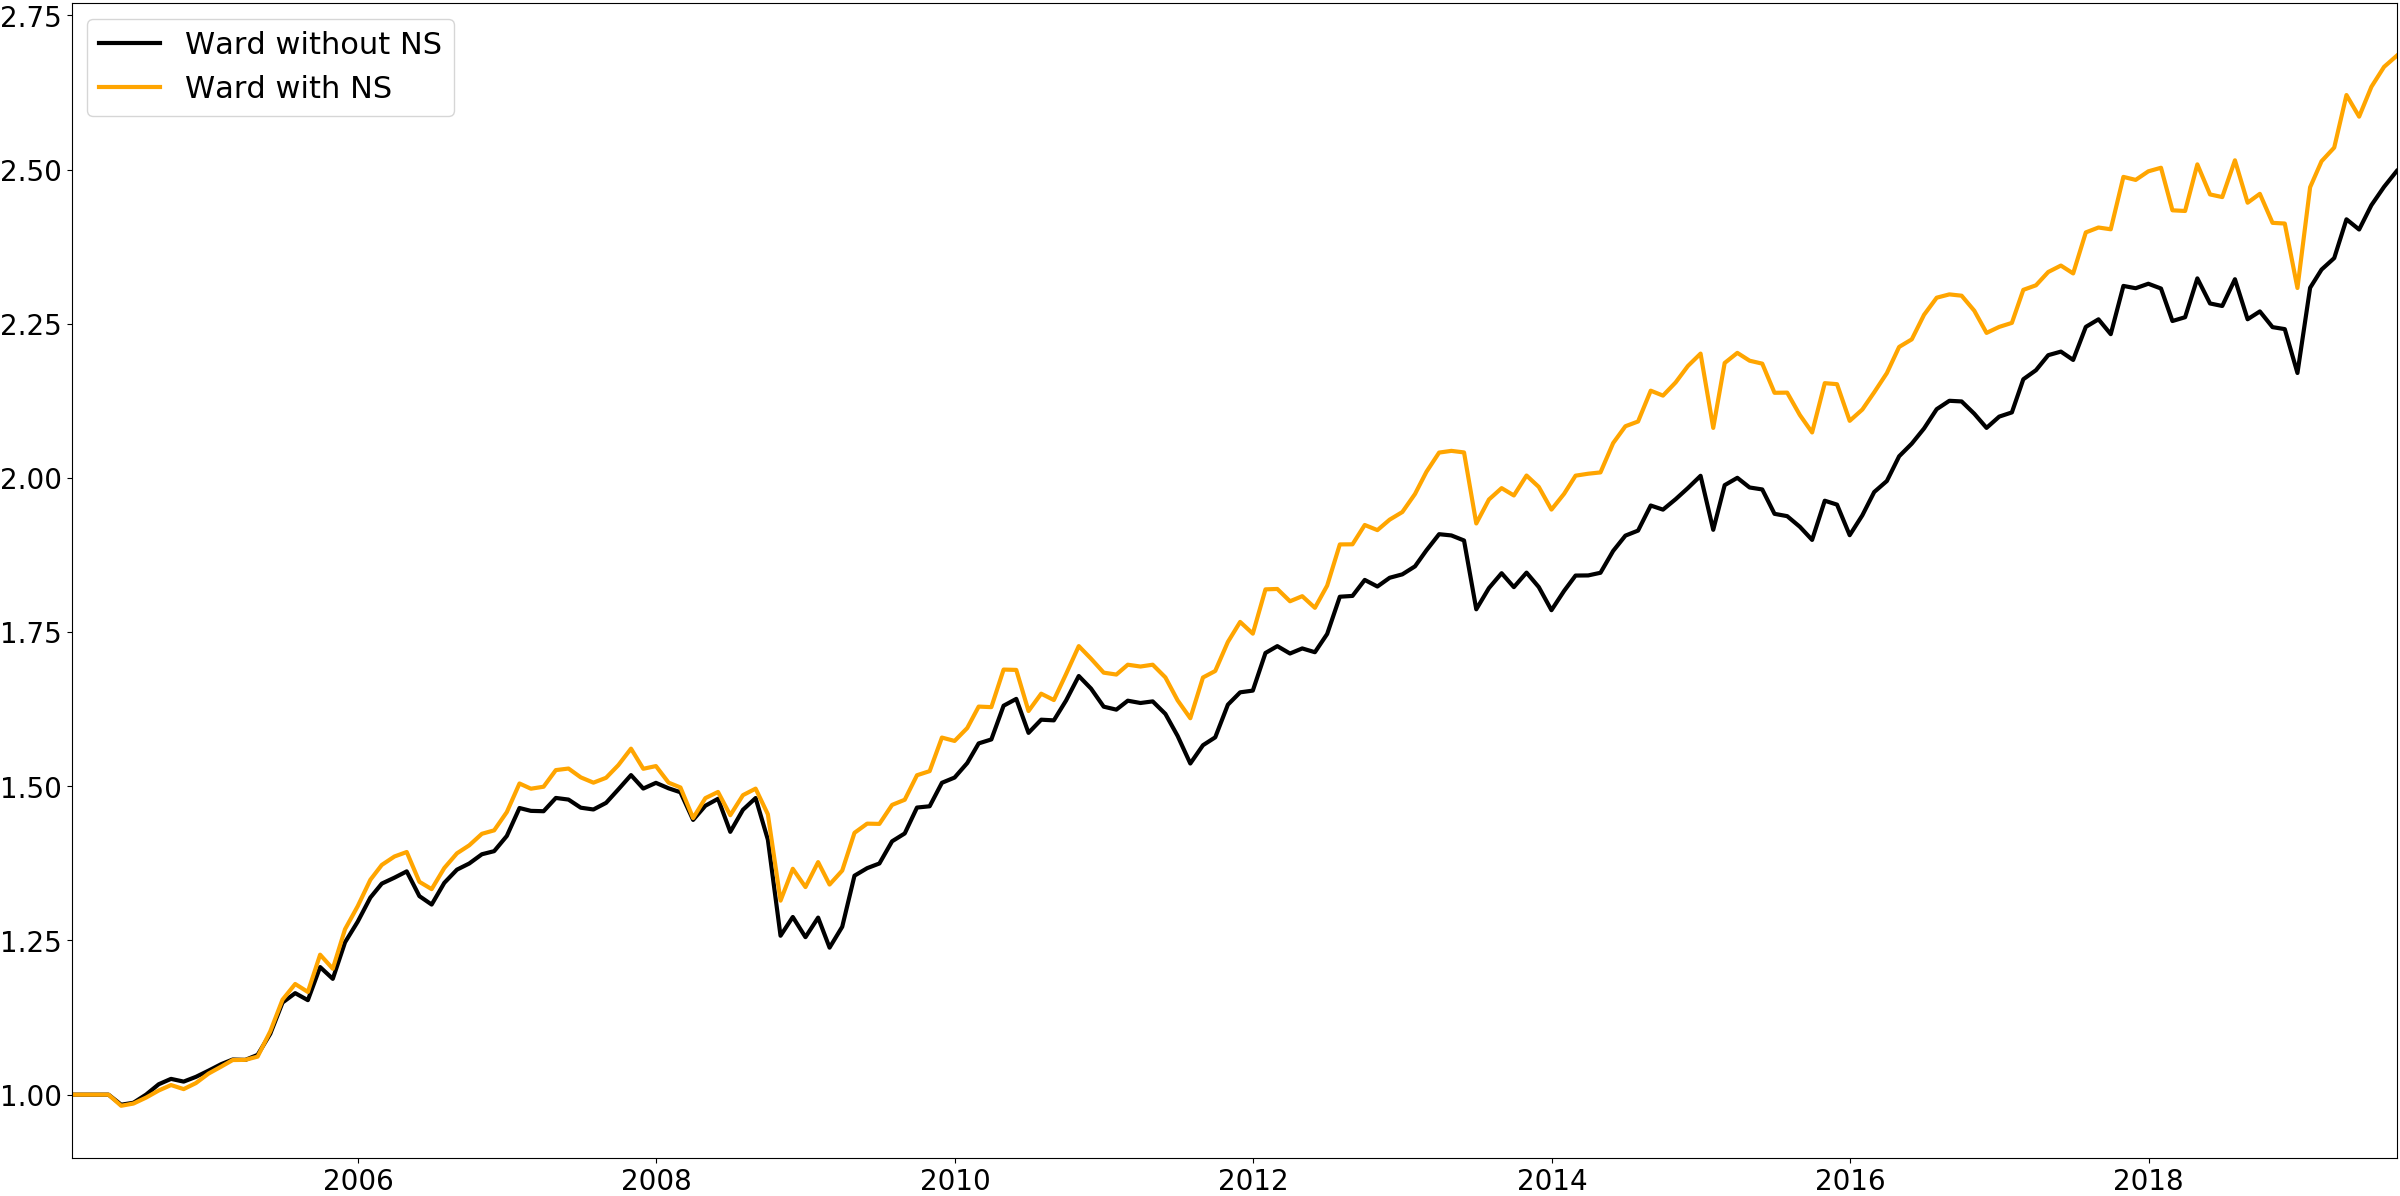
\includegraphics[width=\linewidth]{Plots_and_Tables/perf_noTC_ward_comp_F_2_B_0_LB_12_3_!!}
\caption{Comparison \texttt{ward} clustering approach with and without News Sentiment starting in May 2004.} \label{fig:notc_noNS_perf} % 3 + 2
\end{subfigure}%\hspace*{\fill}

\medskip
\begin{subfigure}{0.8\textwidth}%{0.48\textwidth}
\centering
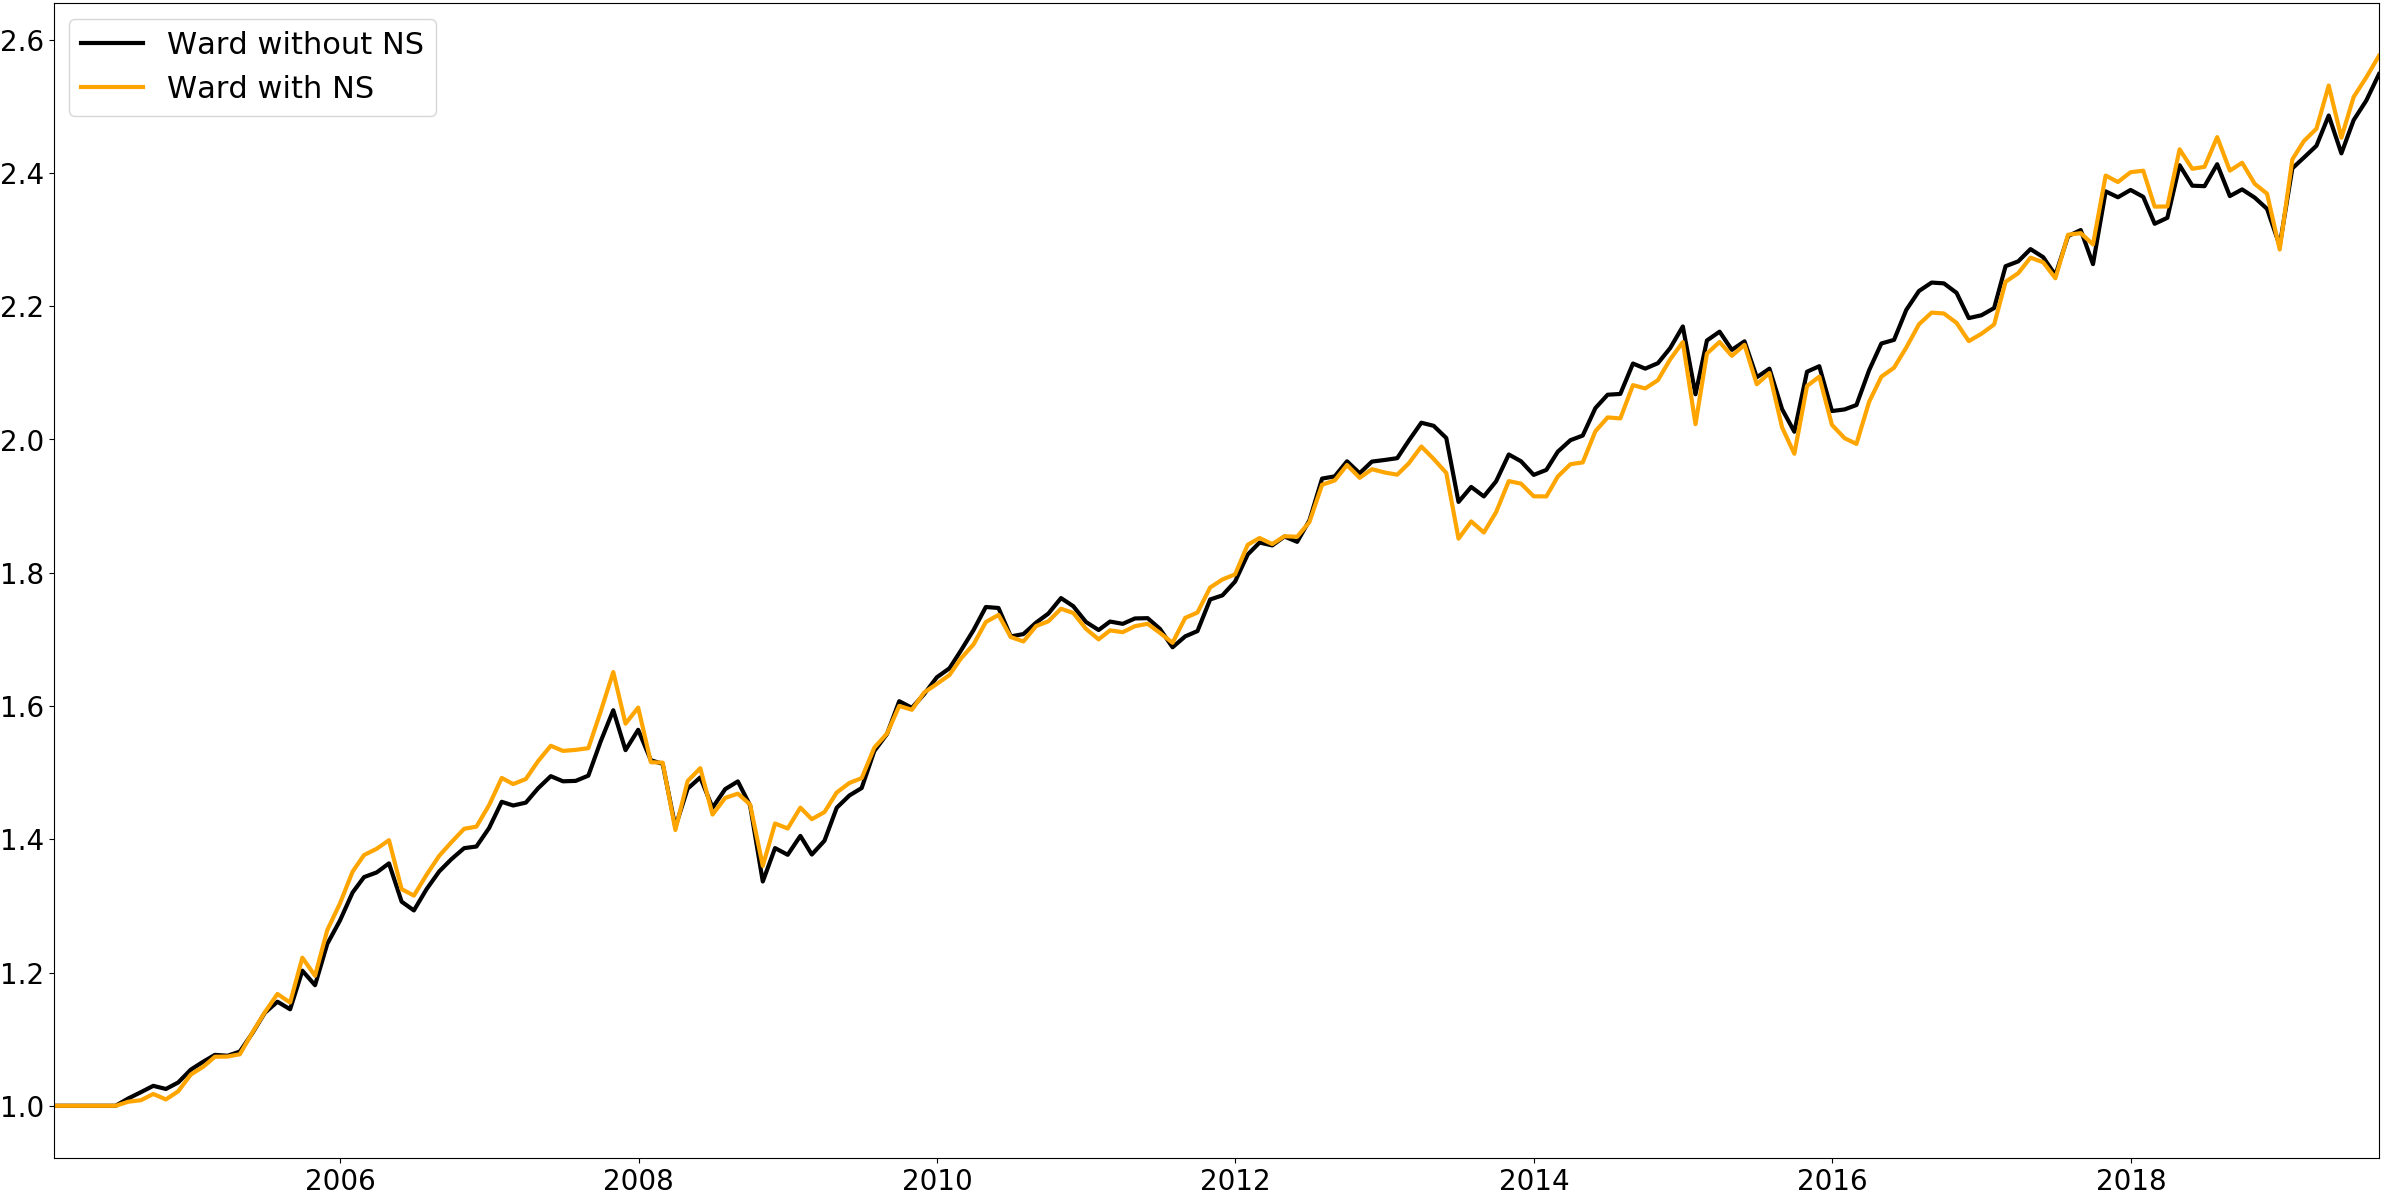
\includegraphics[width=\linewidth]{Plots_and_Tables/perf_noTC_ward_comp_F_2_B_0_LB_12_5_!!}
\caption{Comparison \texttt{ward} clustering approach with and without News Sentiment starting in July 2004.} \label{fig:tc_noNS_perf}
\end{subfigure}%\hspace*{\fill}


\medskip
\begin{subfigure}{0.8\textwidth}%{0.48\textwidth}
\centering
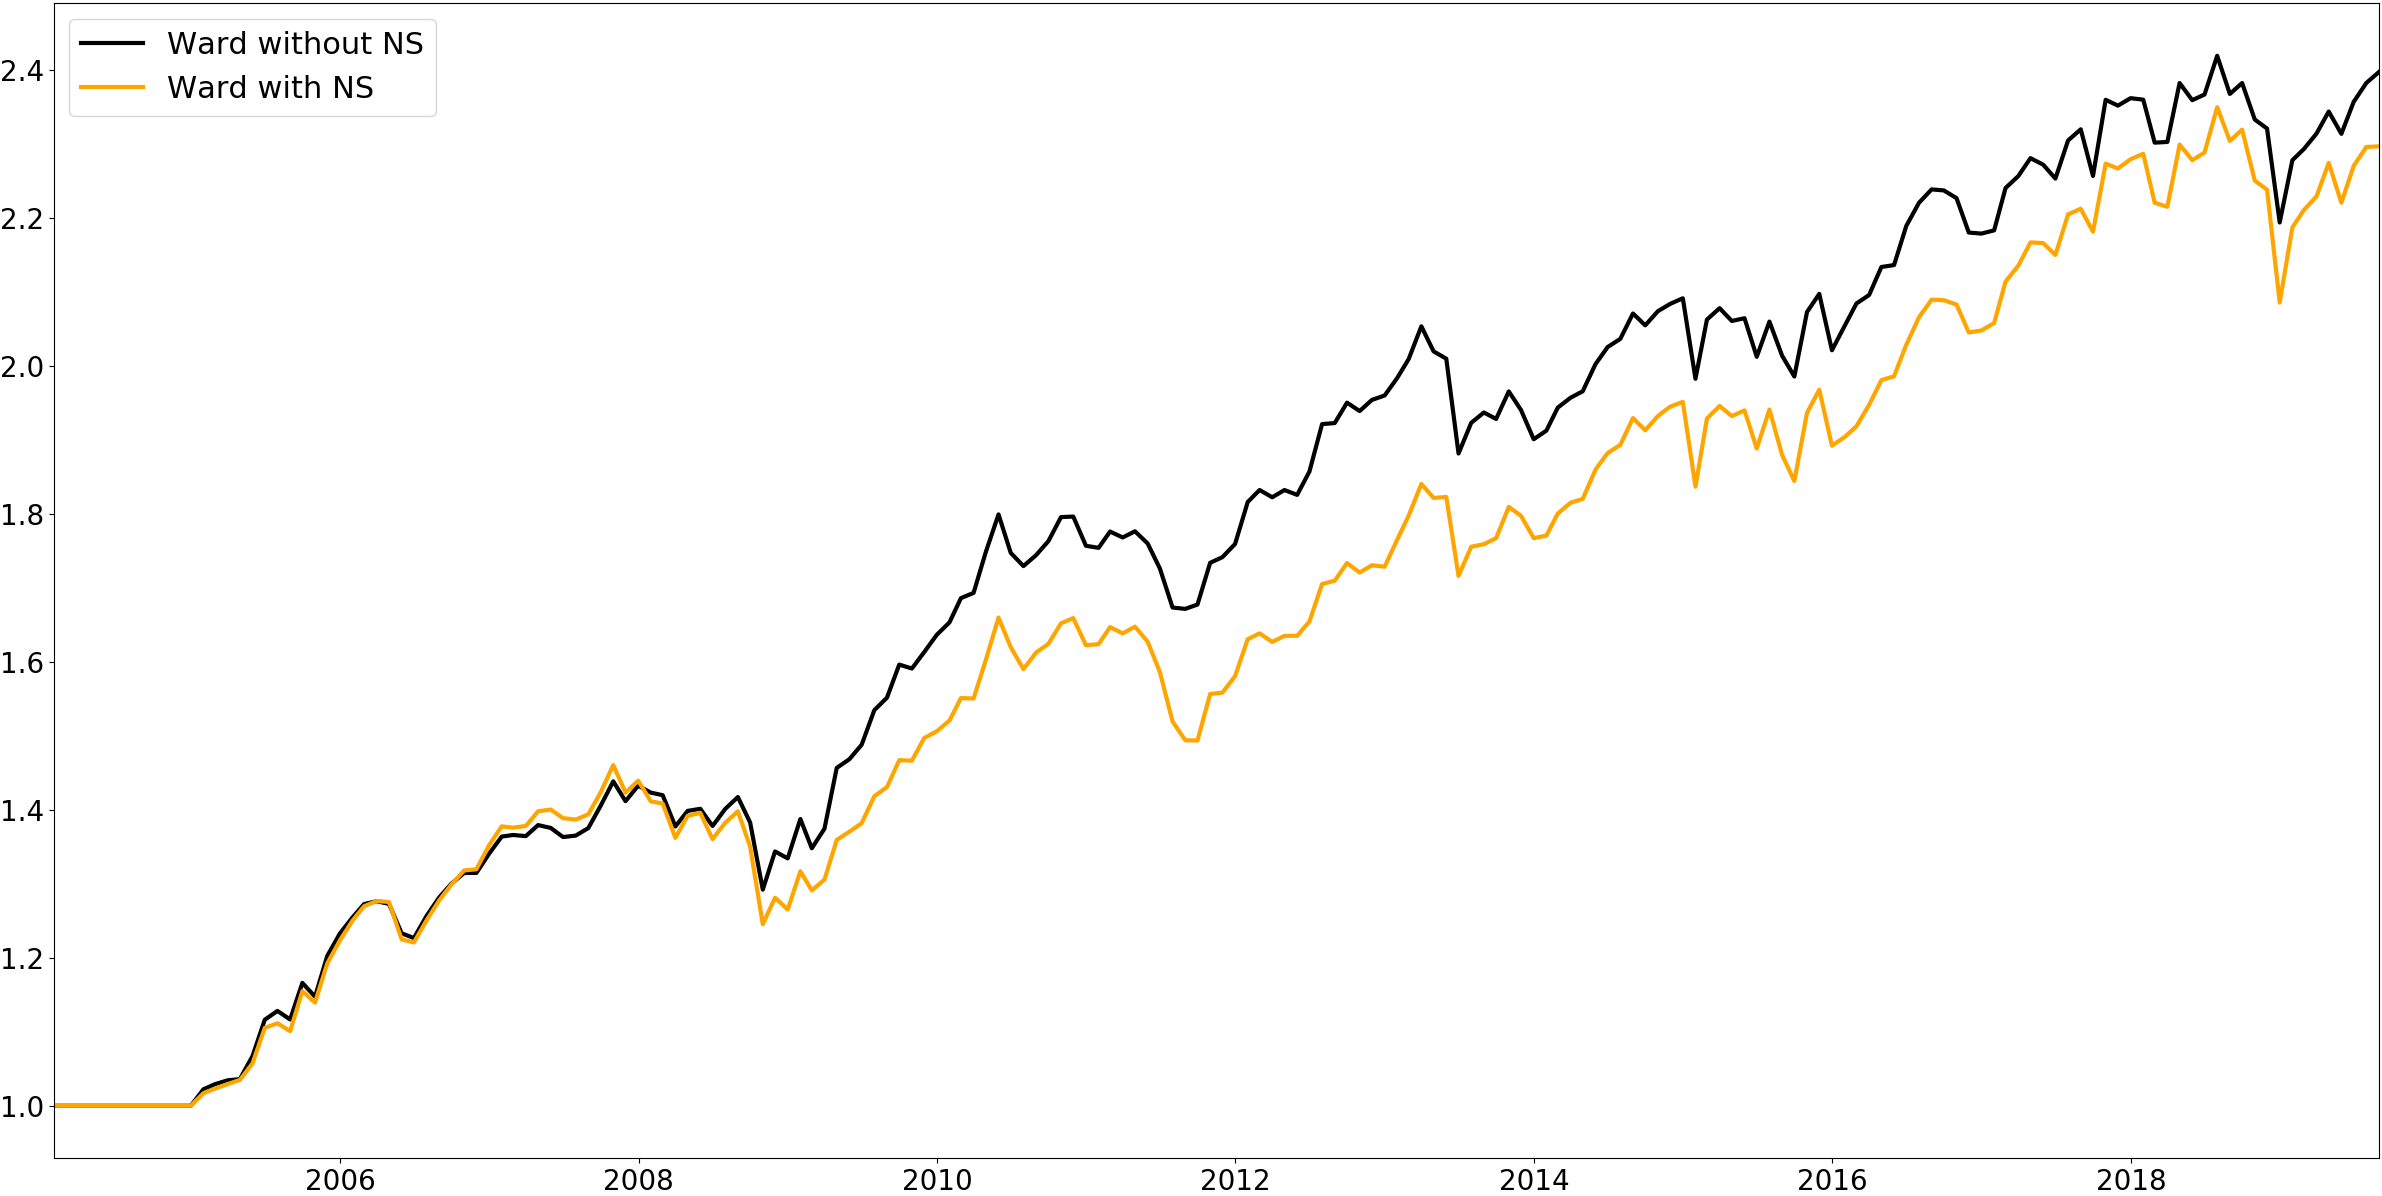
\includegraphics[width=\linewidth]{Plots_and_Tables/perf_noTC_ward_comp_F_2_B_0_LB_12_11_!!}
\caption{Comparison \texttt{ward} clustering approach with and without News Sentiment starting in January 2005.} \label{fig:comp_noNS_perf}
\end{subfigure}%\hspace*{\fill}


\caption{Performance of different strategies without News Sentiment enhancement.} \label{fig:noNS_perf}
\end{figure}
\newpage